\documentclass[11pt, a4paper]{report}

\usepackage{geometry}
\usepackage[utf8]{inputenc}
\usepackage[english]{babel}
\usepackage[T1]{fontenc}

\usepackage{graphicx} % Required for including pictures
\usepackage{float} % Allows putting an [H] in \begin{figure} to specify the exact location of the figure
\usepackage{pdfpages}
\usepackage{booktabs}
\usepackage{tabularx}
\restylefloat{table}
\usepackage{listings}
\usepackage{hyperref}
\usepackage{tikz,pgf}
\usepackage{forest}
\usepackage{caption}
\usepackage{subcaption}
\usepackage{wrapfig} % Allows in-line images such as the example fish picture

\usepackage{lmodern} % load a font with all the characters
\newcommand\tab[1][0.5cm]{\hspace*{#1}}

\linespread{1.2} % Line spacing

%\setlength\parindent{0pt} % Uncomment to remove all indentation from paragraphs

\graphicspath{{Pictures/}} % Specifies the directory where pictures are stored

\renewcommand{\baselinestretch}{1.3}
\headsep = 10.mm
%%%% CHOOSE MARGINS %%%%

\geometry{hmargin=2.5cm,top=3cm,bottom=2.3cm}
%%%% COMMANDS %%%%
%%%%%%%%%%%%%%%%%%%%%%%%%%%%%%%%%%%%% CHANGE HERE %%%%
\renewcommand\title{UCLCampus: a moblie application for UCL students}
\newcommand\nametwo{Arnold \textsc{Moyaux}}
\newcommand\nameone{Baptiste \textsc{Lacasse}}
\newcommand\options{}
\newcommand\supervisor{Yves \textsc{Deville}}
\newcommand\readerone{Kim \textsc{Mens}}
\newcommand\readertwo{Hildeberto \textsc{Mendonça}}
\newcommand\readerthree{Mathieu \textsc{Zen}}
\newcommand\readerfour{Jorge \textsc{Perez Medina}}
\newcommand\years{2015-2016}
%%%% BEGIN %%%%
\begin{document}

%%%% COVER %%%%
\thispagestyle{empty}
\noindent\begin{minipage}{.25\textwidth}
\noindent
\includegraphics[width=3.6cm]{Images/ucl.jpg}
\end{minipage}
\begin{minipage}{.5\textwidth}
\begin{center}
UNIVERSITE CATHOLIQUE DE LOUVAIN
\\~\\~
ECOLE POLYTECHNIQUE DE LOUVAIN
\\~\\~\\~\\~\\~
\end{center}
\end{minipage}
\begin{minipage}{.25\textwidth}
\hfill
\includegraphics[width=3.6cm]{Images/epl.jpg}
\\~\\~\\~\\~
\end{minipage}
\vspace{4.5cm}
\begin{center}
\bfseries{\scshape{\Huge{\title}}}
\end{center}
\vspace{4.5cm}
\begin{minipage}{.5\textwidth}
\begin{tabular}{ll}
Supervisor: & \supervisor
\\ Readers: & \readerone 
\\          & \readertwo 
\\          & \readerthree
\\          & \readerfour
\end{tabular} 
\\~\\~
\end{minipage}
\begin{minipage}{.5\textwidth}
\begin{tabular}{l}
Thesis submitted for the Master's degree
\\ in computer science and engineering
\\ by : \nameone
\\ 	   \nametwo
\end{tabular}
\end{minipage}
\vfill
\begin{center}
Louvain-la-Neuve
\\ Academic year \years
\end{center}
%%%% END COVER %%%%
%----------------------------------------------------------------------------------------
%	TABLE OF CONTENTS
%----------------------------------------------------------------------------------------

\tableofcontents % Include a table of contents
\newpage % Begins the essay on a new page instead of on the same page as the table of contents 


\chapter{Introduction} % Major section

Brief introduction of the project, the goals and the contents of the rest of the thesis.


\chapter{Background}

In this section, we will look at the different existing technologies relating to the different aspects of our project and will explain the choices we made. // TODO

\section{Cross-platform mobile development tools}

In each of these sections, we will detail the different approaches one could choose to develop a cross-platform moblie applications. We will also present several frameworks using these approaches. We will then compare them and choose one of those approaches for the rest of the project. //TODO
\subsection{The native approach}

The first approach we considered for our project was what we call a native approach. The native approach consists in using the native technology and language for each platform, for instance Java for Android and Objective-C for iOS.  

\begin{table}[H]
\begin{tabularx}{\linewidth}{>{\parskip1ex}X@{\kern4\tabcolsep}>{\parskip1ex}X}
\toprule
\hfil\bfseries Pros
&
\hfil\bfseries Cons
\\\cmidrule(r{3\tabcolsep}){1-1}\cmidrule(l{-\tabcolsep}){2-2}

Best achievable performance\par
Always up-to-date with the latest API\par
Can use any platform\par

&

Low maintainability\par
Harder to find contributors fluent in all technologies\par
Can lead to different versions of the application\par


\\\bottomrule
\end{tabularx}
\caption{Pros and cons of the native approach}
\end{table}

\subsection{The web approach}
A second approach we considered was the web approach. This approach consists in using HTML5 to develop an application that will be usable on any platform.


\begin{table}[H]
\begin{tabularx}{\linewidth}{>{\parskip1ex}X@{\kern4\tabcolsep}>{\parskip1ex}X}
\toprule
\hfil\bfseries Pros
&
\hfil\bfseries Cons
\\\cmidrule(r{3\tabcolsep}){1-1}\cmidrule(l{-\tabcolsep}){2-2}

Can be used on any mobile platform\par
Easy to find contributors fluent in HTML5\par
Easy to maintain\par

&

Doesn't have access to native platform features\par
Harder to implement local storage/security (//TODO NEED BETTER SOURCE)\par
Not as performant as native\par



\\\bottomrule
\end{tabularx}
\caption{Pros and cons of the web approach}
\end{table}
\subsection{The hybrid approach}

The last approach to develop a mobile application is called the hybrid approach. An hybrid app is mostly built using HTML5 and JavaScript and is then wrapped inside a thin native container, giving it access to native features.

\begin{table}[H]
\begin{tabularx}{\linewidth}{>{\parskip1ex}X@{\kern4\tabcolsep}>{\parskip1ex}X}
\toprule
\hfil\bfseries Pros
&
\hfil\bfseries Cons
\\\cmidrule(r{3\tabcolsep}){1-1}\cmidrule(l{-\tabcolsep}){2-2}

Can be used on any mobile platform\par
Easy to find contributors fluent in HTML5 and JavaScript\par
Easy to maintain\par

&

Not as performant as native\par



\\\bottomrule
\end{tabularx}
\caption{Pros and cons of the hybrid approach}
\end{table}

\subsection{Our choice}

\section{Open-source project and code sharing}

In this section, we will explain the choices we made concerning the code sharing platforms we used as well as the licenses we used to protect our work.

\section{Project Management Methodologies}

Here we detail the choices we made as to how we were going to manage the different parts of the project.

\chapter{Functionalities of UCLCampus}

In this chapter, we will show how we defined the relevant functionalities of our application as well as the user interface.

\section{Choice of functionalities and sections}


In order to define what kind of functionalities we wanted to be part of our application, we needed to know what the students needed. The first step was to define a number of user stories that we would then translate into functionalities.\\ 
We split our user stories into several categories:

\begin{itemize}

\item Studies: anything directly related to a user's studies, for instance his classes, the lecture halls or the libraries.
\item Campus: anything related to student life in the campus but not related to the user's studies. For instance "Kot à Projets" or "Cercles".
\item City: anything related to the city the user is in but not related to the university. For instance a cinema or restaurants.
\item Tools: the tools offered by the application that might relate to several other categories. For example the map.
\item Settings: the settings of the application. For example the language or the currently selected campus.

\end{itemize}

We also define two types of users:

\begin{itemize}

\item Students: students can access all the functionalities of the application using their UCL login information. Indeed, some functionalities are student specific. For instance, it wouldn't make sense for a person who isn't a student to try to access his or her schedule.

\item Users: users are people who aren't students but might still be interested in some functionalities the application has to offer. 

\end{itemize}

In our user stories, any story starting by 'as a student' cannot be used by users while any story starting by 'as a user' can be used by both users and students.\\

We will now give a list of the different user stories we thought of for each of our categories.

\subsubsection{Studies}

\begin{itemize}

\item Schedule
\begin{itemize}
\item As a student, I can access my schedule in order to know when my courses are given.
\item As a student, I want to know where a course is given.
\item As a student, I want to know the name of a teacher giving a certain course of my schedule.
\item As a student, I can export my schedule to my phone's agenda so that I don't need Internet access to see it.
\end{itemize}

\item Libraries
\begin{itemize}
\item As a user, I can see whether a library is open or closed.
\item As a user, I can display the address of any library.
\item As a user, I can have a GPS guide to access libraries from my location.
\end{itemize}

\item Lecture halls
\begin{itemize}
\item As a user, I can check the address of any lecture hall.
\item As a user, I can have a GPS guide to access lecture halls from my location.
\end{itemize}

\item Websites
\begin{itemize}
\item As a user, I can quickly access the moodle website through the application.
\item As a user, I can quickly access the UCL website through the application.
\end{itemize}

\end{itemize}

\subsubsection{Campus}

\begin{itemize}

\item{Events}
\begin{itemize} 
\item As a user, I can see a list of events taking place in my campus.
\item As a user, I can sort the events by category.
\end{itemize}

\item{Kots à Projet}
\begin{itemize}
\item As a user, I can check Kots à Projet to know their address and projects.
\item As a user, I can have a GPS guide to access Kots à Projet from my location.
\end{itemize}

\item{Cercles}
\begin{itemize}
\item As a user, I can check "Cercles" to know their address.
\item As a user, I can have a GPS guide to access "Cercles" from my location.
\end{itemize}

\item{Restaurants Universitaires}
\begin{itemize}
\item As a user, I can see the different "Restaurants Universitaires" in my campus.
\item As a user, I can check the menu of the "Restaurants Universitaires".
\item As a user, I can have a GPS guide to access "Restaurant Universitaires" from my location.
\end{itemize}

\item{Sports}
\begin{itemize}
\item As a user, I can see a list of sports organized in my campus.
\item As a user, I can sort the sports by day or by sport.
\end{itemize}

\end{itemize}

\subsubsection{City}

\begin{itemize}

\item Tourism
\begin{itemize} 
\item As a user, I can see the address of the city's information center.
\item As a user, I can see a list of the museums of the city I'm in.
\item As a user, I can see whether a museum is opened or closed.
\end{itemize}

\item Activities
\begin{itemize} 
\item As a user, I can see the address of the city's cinema in order to access it with the help of a GPS guide.
\item As a user, I can see several activities I can do in the city I'm in.

\end{itemize}

\item Restaurants and bars
\begin{itemize} 
\item As a user, I can see a list of the restaurants of the city I'm in.
\item As a user, I can see a list of the bars of the city I'm in.
\end{itemize}

\end{itemize}

\subsubsection{Tools}

\begin{itemize}
\item Maps
\begin{itemize}
\item As a user, I can access a map of the city I'm in in order to check points of interests.
\item As a user, I can receive help from a GPS guide in order to access a location of my choice on the map.
\end{itemize}
\item Mail
\begin{itemize}
\item As a student, I can check my emails on my uclouvain account.
\item As a student, I can send emails from my uclouvain account.
\end{itemize}
\item{Help}
\begin{itemize}
\item As a user, I can see where the UCL parkings are located.
\item As a user, I can receive help about how to configure the UCL wifi.
\item As a user, I can receive help about common transportation.
\end{itemize}
\end{itemize}

\subsubsection{Settings}

\begin{itemize}
\item As a user, I can change the application's language to French, English or Dutch.
\item As a user, I can select my campus.
\item As a student, I can login on my UCLouvain.be account.
\item As a student, I can log out from my UCLouvain.be account. 
\end{itemize}

\section{User interface}

Once we determined the different features we wanted in our application, we needed to organize them in a way that makes sense for users. In order to do so, we made sketches of what the application might look like using InVision. InVision is a website that lets people design and style mobile applications prototypes. It allows us to get an idea of what the finished product might look like without having to dive into any code. The sketches we made are available in the annex.\\

In these sketches, we can see that we decided to have one menu per category we defined in the previous section. Each menu has an associated color, allowing the user to always have visual clues to help them know where they are.\\

Once the sketches were done, we shared the link to our prototype to over 1000 students, mostly student in their first year, as they represent the future users of this application. They were able to browse through the application using the buttons, as if it was already working, and leave comments and feedback wherever they wanted to.\\

While we didn't receive as much feedback as we would have hoped, the one we received was constructive and helpful. Most people were satisfied with our 3 first categories, Studies, Campus and City. The fourth category, however, was more criticized. Here are some comments we received concerning the Tools category.\\

\iffalse
\say{[...]\\ 
 -Quelques remarques:
 -\begin{itemize}
 -\item L'icône "Outils" du menu principal pourrait être renommer par soucis de clarté, on s'attend à tomber sur les "outils" ou paramètres de l'application et non pas du campus/ de la ville.
 -\item Je ne vois pas trop l’intérêt de l'onglet mail étant donné que la plupart des étudiants possédant un smartphone ont déjà leur boite mail étudiant connectée. 
 -\item L'onglet "Aide" est un peu caché et on ne s'attend pas à trouver ces infos là quand on clique, le lien parking devrait plutôt figurer dans le menu "ville" par exemple. (le renommer "infos utiles", ou qqch de plus parlant que "aide" éventuellement).
 -\end{itemize}
 -[...]}\\\\
 -\say{[...] \\
 -2. la partie "mails" est sans intérêt puisqu'on est sur un smartphone où la messagerie est probablement déjà configurée.\\
 -3. le menu "Aide" pourrait alors remonter d'un niveau et remplacer "Outils" qui n'est d'ailleurs pas très parlant comme titre de menu}\\
 \fi

After reading these comments, we decided to rework the Tools section. We agreed that the mail part was superfluous and we decided to drop it entirely. We also decided to drop the "Help" section as we didn't think it was important enough. That left us with the map. We decided that it was important that the map was not grouped with the city, the studies or the campus as it was important to all three sections. We thus decided to leave it in the Tools section. We also decided against renaming the section "Maps" as future contributors may very well add functionalities we didn't think of in this section.
\chapter{Implementation}


Here we will explain the overall architecture of the application. We will also explain some aspects we considered when implementing the application.

\section{Architecture}

The purpose of the application is to be extensible and easily maintainable. We wanted a programmer to have the possibility to add his functionalities at each level of the application.
For this we thought our implementation as a tree. At the top level we have the generic parts and configurations that will be everywhere in the application under it we have the settings menu and next to it we have four branches pointing to global sections that we decided to create, themselves pointing to their functionalities and so on. Here is a part of the tree in order to give you the idea.\\

\begin{forest}
[Application, for tree = {ellipse, draw}, fill = green
	[Settings]
	[Studies]
	[Campus
		[Events]
		[Cafeteria
			[Menu]		
		]
		[Cercles]
		[Sports]
	]
	[Tools]
	[City]
]
\end{forest} 

\subsection{Folder organisation}
We wanted to keep the same state of mind for the file organisation. Ionic base architecture is to put all html file in a folder named templates, all js in a JS folder, ... The problem is that become messy once we have a lot of functionalities(thus a lot of files). We modify it to respect the tree architecture we want. With our folder system, a programmer can add his own subtree to the main tree. And if you want to modify a specific functionality, you have directly access to the related files. Figure 4
1 is a summary of the change, red folder are those we modify.
\begin{figure}
\centering
\begin{subfigure}[b]{0.5\textwidth}
   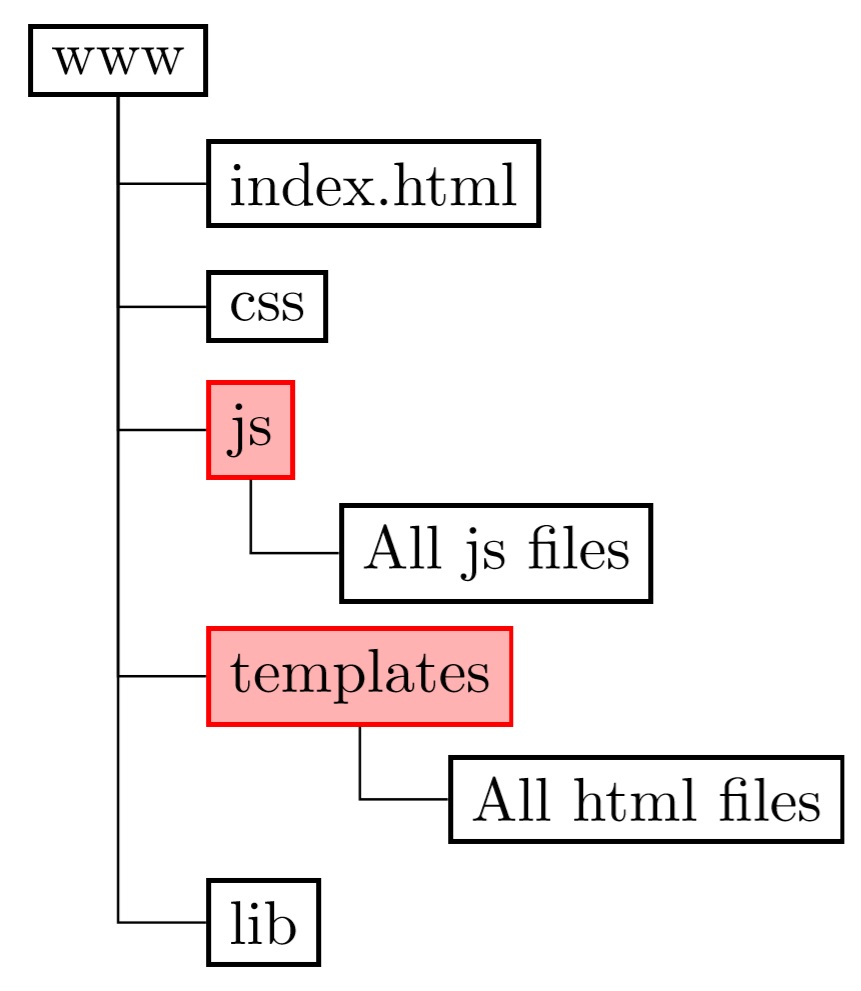
\includegraphics[width=.4\linewidth]{Images/folder_before.jpg}
  \caption{Before}
  \label{fig:before}
\end{subfigure}%
\begin{subfigure}[b]{.5\textwidth}
  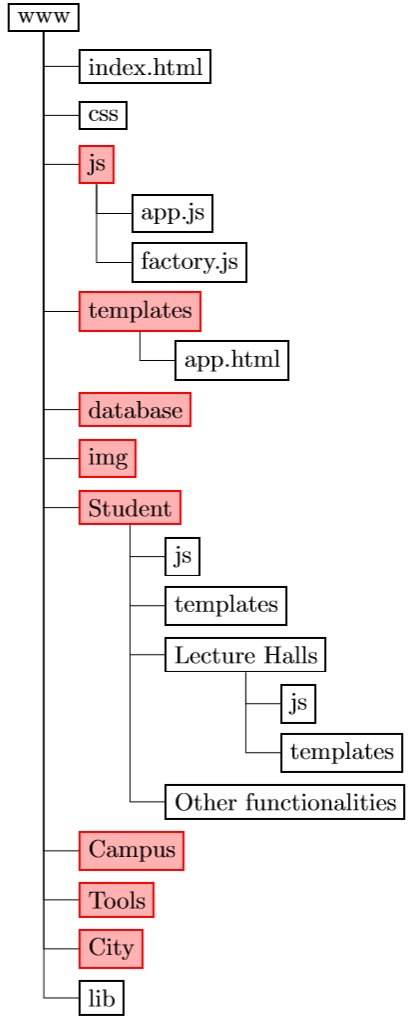
\includegraphics[width=.4\linewidth]{Images/folder_after.jpg}
  \caption{After}
  \label{fig:sub2}
\end{subfigure}
\caption{Folder evolution}
\label{fig:test}
\end{figure}

\subsection{Information processing}

Here I just explain how we deal with the information processing from an architecture's design point of view. The section 4.4 explains in detail how we did it for each specific part.
There is a lot of external information to relay into the application (libraries schedule, libraries addresses, daily events in the campus,...). We have two possible ways to import them.

\subsubsection{Database}

\begin{table}[H]
\begin{tabularx}{\linewidth}{>{\parskip1ex}X@{\kern4\tabcolsep}>{\parskip1ex}X}
\toprule
\hfil\bfseries Pros
&
\hfil\bfseries Cons
\\\cmidrule(r{3\tabcolsep}){1-1}\cmidrule(l{-\tabcolsep}){2-2}

Always available\par
Easy information retrieval(query)\par
Easy to modify\par
Fast\par

&

Need someone to update\par
Takes memory \par


\\\bottomrule
\end{tabularx}
\caption{Pros and cons of a database}
\end{table}

\subsubsection{Web parsing}

\begin{table}[H]
\begin{tabularx}{\linewidth}{>{\parskip1ex}X@{\kern4\tabcolsep}>{\parskip1ex}X}
\toprule
\hfil\bfseries Pros
&
\hfil\bfseries Cons
\\\cmidrule(r{3\tabcolsep}){1-1}\cmidrule(l{-\tabcolsep}){2-2}

Automatic update\par
Easy information retrieval with web services(query)\par
No hardware memory consumption\par

&

Need an Internet connexion and an operational server side\par
Horrible information retrieval without web services\par
If the web server change, maybe you will need to recode all the parsing method\par
Slow\par


\\\bottomrule
\end{tabularx}
\caption{Pros and cons of the web parsing}
\end{table}


An considerable limitation is the need for someone in order to update the database or creating new parsing system. We have no workforce for it, so if we have the choice between the two methods, we will select the one needing less modification in the future.

\subsection{Front-end and back-end}

\begin{itemize}
\item Front-end: Part of the user interface that can be separated in two fields. First is design and the second is html, css and JavaScript development.
\item Back-end: Is the hidden part of the iceberg, what you can't see. For example: the database, the parsing function, ...
\end{itemize}

We create a front-end and a back-end system in our application. It helps a lot for the maintain because you can modify part without involving the other. For example, we store lecture halls in the database but the UCL create a new website with web services providing all lecture halls and their information. It's better than the database because it automatically updates and so you want to use them instead. You can do it in a specific part that is totally isolated from the code for the user interface.	

\subsection{Factory}

Factory is a functionality from angularjs which we used as a back-end service. The factory will take the data from the database or web parsing, modify the data format to be easier to handle and then transmit it to the front-end. Figure 4.2 illustrates this.\\

\begin{figure}
\centering
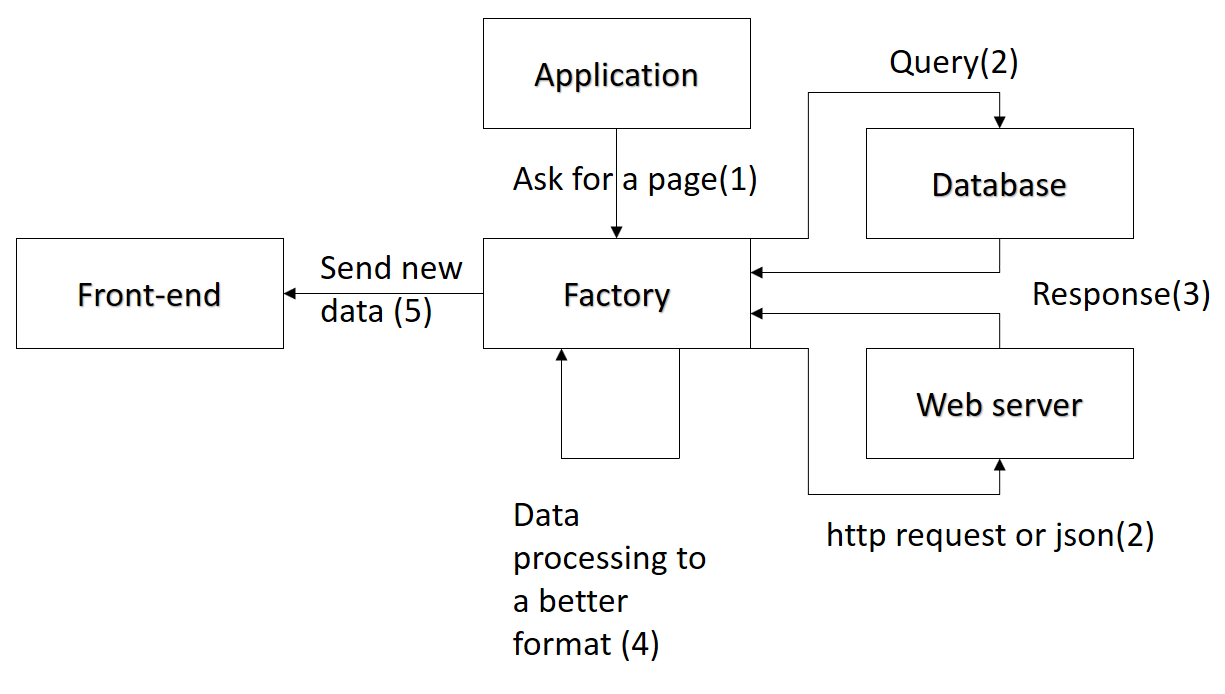
\includegraphics[scale = 0.3]{Images/factory_arch.png}
\caption{Factory operation}
\end{figure}

For example, we open the page for the schedule. (1)the system notifies the schedule factory in order to get his data. (2) the factory create a custom HTTP request and send it to the ADE domain. (3) Server sends a response. (4) Data in the response are not easy to manipulate (long string with html tags inside), so the factory pick the important element in the response(with a parsing algorithm) and put them in a JavaScript object where data are easy to handle. (5) Send new data to front-end.

\subsection{State provider}

The state provider is a functionality of angularjs. It allow you to define the page configuration (cached or not for example). Furthermore it create an edge between the back end and the front end, figure 4.3 illustrate the operation of the state provider. 
\begin{figure}[H]
\centering
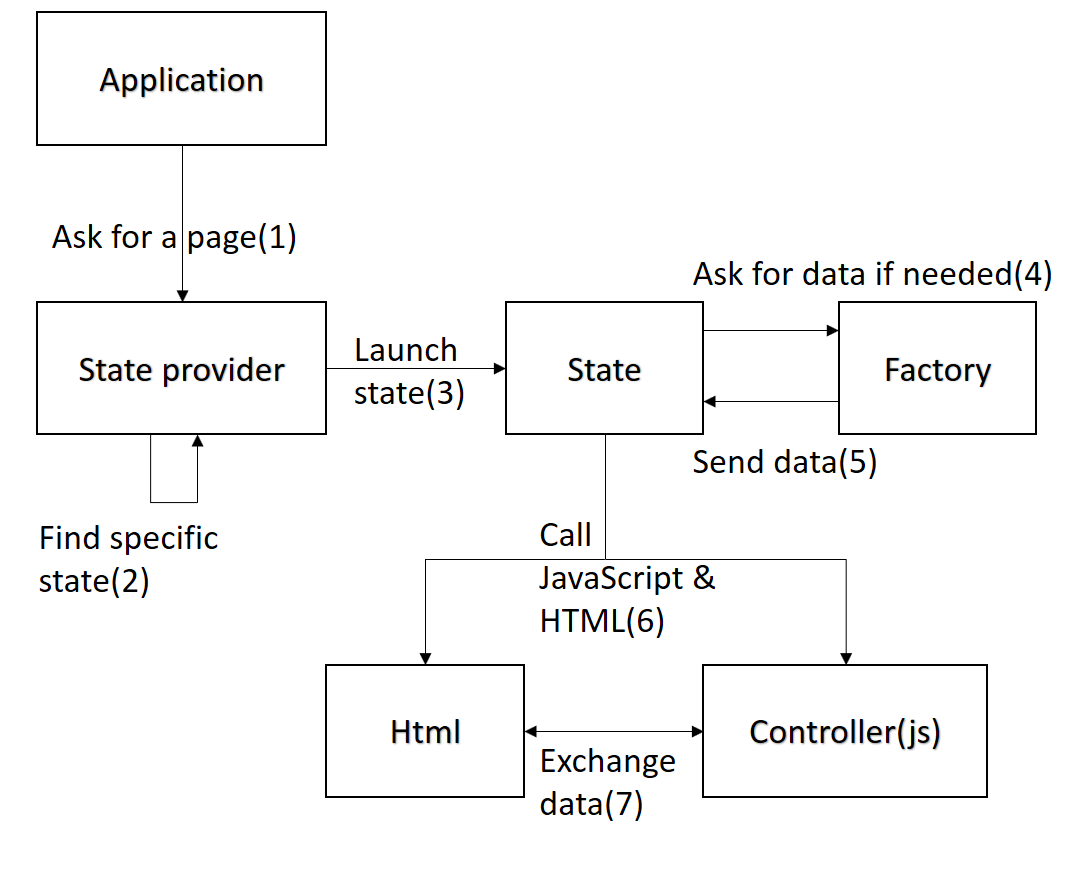
\includegraphics[scale = 0.3]{Images/stateProvider_arch.png}
\caption{State provider operation}
\end{figure}
First the application ask for a page. The state provider contain a list of specific state(one state by page), it will return the state relative to the asked page. The state will contain information about the page:
\begin{itemize}
\item The location of the html template
\item The associate controller(js)
\item A flag for cache memory(true or false)
\item The tab membership(for example student if we are in the subtree student)
\end{itemize}. For back end data(optional), the state will call the needed factory and wait its response before launching the template and the controller for the user interface. JavaScript(controller) and Html can exchange informations and sent it to back end in some cases.
\iffalse
\begin{lstlisting}
.state('app.name', {
    cache:{true or false},
    url: "/url name",
    views: {
      'appropriate-tab': {
        templateUrl: "html file",
        controller: "page controller(javaScript)",
        resolve:{
          facotry: function(Factory) {
            return Factory.neededData();
          }
        }
      }
    }
  })
\end{lstlisting}
\fi
\section{Coding standards}
\subsection{Header and footer}
We managed our code to create automatically a default new footer and header when you start new html template. The footer and header have a specific color for each tab-section (blue for student, yellow for campus, purple for tools and green for town). We allow developers to overwrite the default header but under two condition
\begin{itemize}
\item The title have to keep the same font and have to be center.
\item The header color must respect the section color
\end{itemize}
Footer must not be overwrite or be hidden. If developers need to insert their specific header or footer, Ionic provide a css in order to add subfooter and subheader.
\subsection{Tree hierarchy}
We want developers to keep the tree hierarchy we created for the state and for the folder. For css and extra JavaScript, html, we don't enforce any rules as long as it stay in the relative module.
\subsection{Colors}
We used the UCL colors code\footnote{https://www.uclouvain.be/459461.html}. For this we modified the sass theme of Ionic. This allow module developed with basic ionic css component to update with the application color instantly and automatically. The main color of UCLCampus is the blue "UCL".

\begin{center}
    \begin{tabular}{ | c | c | c |}
    \hline
    Color & css name & code\\ \hline
    Blue & positive & \#00214e\\ \hline
    Yellow & energized & \#f29400\\ \hline
    Purple & royal & \#88005d\\ \hline
    Green & balanced & \#76ad1c\\ \hline
    \end{tabular}
\end{center}

\section{Security}



\section{Information retrieval}

In this section we will detail the different sources of information we used in our application as well as the technologies we had to use in order to retrieve said information. 

\subsection{Libraries and lecture halls}

In order to retrieve a list of all libraries and lecture halls in the university, we contacted the UCL to ask them if such a database existed. Sadly, it appeared that no database of this kind exists. We then wondered how LLNCampus //TODO parler de LLNCampus avant// managed to obtain all the information they had on lecture halls and libraries. Since their application is also open-source, we were able to find the database they used. Since it was very complete and was the only database available, we decided to re-use this database. However, since their database was built with only one campus in mind, we had to change it a bit.

\subsubsection{Database structure}
 
//TODO include er diagram ? useful ?
The database is an SQLite database. The table we use for the most part is called "poi" (point of interest) and has the following fields:

\begin{itemize}
\item ID (integer): used to identify the item
\item Name (text): name of the point of interest
\item Latitude (real): latitude of the point of interest
\item Longitude (real): longitude of the point of interest
\item Type (text): type of the point of interest, can be "auditoire", "kap",   "bibliotheque", ...
\item Address (text): address of the point of interest
\item Img (text): path to the image linked to the poi
\end{itemize}

To these fields we added the following two:
\begin{itemize}
\item Campus (text): campus where the poi is located
\item Abbr (text): abbreviated version of the poi. For instance "BARB" for the Ste-Barbe lecture hall
\end{itemize}

The first field is useful if we want to have different campuses (//TODO check orthographe) while the second is used to find the poi on the map.

\subsubsection{Retrieving lecture halls}

Once we had the completed the database, we had to connect it to our application. In order to do so, we used the cordovaSQLite plugin. Once connected, we were able to retrieve the lecture halls using the following SQL query: 
\begin{verbatim}
SELECT * FROM poi WHERE TYPE = 'auditoire' AND CAMPUS = ?
\end{verbatim}

This query will retrieve all the fields from the poi table we discussed earlier which have the type "auditoire" and are located in the desired campus. The "?" character is used as a placeholder for an argument we can pass to the function. We will then store the result of the query in a JavaScript array and used that array to display the information to the user.

\subsubsection{Retrieving libraries}

In order to retrieve all the information concerning libraries, the poi table was not enough. Indeed, we wanted the users to be able to know whether a library was opened or closed and the schedule was not available in the poi table. Thankfully this information was available in another table, called "bibliotheque\textunderscore horaire". This table only has 4 fields:

\begin{itemize}
\item Building\textunderscore ID (integer): identifies the library. Same id as the one used in the poi table.
\item Day (integer): Day of the week (0 for monday, 1 for tuesday, ...)
\item Begin\textunderscore time (integer): Time of the day when the library opens. Given in minutes elapsed since midnight
\item End\textunderscore time (integer): Time of the day when the library closes. Given in minutes elapsed since midnight
\end{itemize}

Given this new table we were able to retrieve all the information we needed using the following SQL query:
\begin{verbatim}
SELECT * FROM poi, bibliotheque_horaire WHERE poi.TYPE = 'bibliotheque' 
AND poi.ID == bibliotheque_horaire.BUILDING_ID AND DAY = ? AND CAMPUS = ?
\end{verbatim}

This query retrieves all poi with type "bibliotheque" and finds their respective schedule for a given day, all that for a given campus. The result in then stored in a JavaScript array.

\subsection{Events}

In order to find events taking place in Louvain-la-Neuve, we used the www.louvainfo.be website. This website provides a schedule of all upcoming events in the city. It is however specific to Louvain-la-Neuve and we would need to find equivalent websites for the other campuses. \\ The website provides an Atom RSS feed of the events. We decided to use Yahoo Query Language to parse the RSS feed and retrieve the information. The reason we used the Yahoo Query language was that it was the only way we found to perform such an operation. Indeed, the more widely used Google Feed API has been deprecated. We therefore had no other choice but thankfully we haven't encountered any issue with YQL.\\
\\We used the following query to retrieve the feed:
\begin{verbatim}
select * from feednormalizer where url='http://louvainfo.be/evenements/feed/calendar/'
\end{verbatim}
The result is then parsed and stored in a JavaScript array. 


\subsection{Schedule}
For the schedule we had no choice between database or web parsing. The ADE dump database for all courses(of all the students) has a size of 70mb which is way too much memory for a mobile application. Therefore ADE has a custom web site where you are able to send customize url in order to extract specific informations. It's a bit worse than web services because you need a parsing technique.
\subsubsection{ADE custom URL}
The request always start with \url{http://horairev6.uclouvain.be/jsp/custom/modules/plannings/direct_planning.jsp?}. After it we can add some query parameters.
\begin{itemize}
\item code : The course code we want to see on the schedule. We picked the logged student courses codes for it.
\item weeks : The weeks we want to see. It's a number per weeks. We wanted to get all the year so we used a suite from 1 to 52 (1,2,3,...).
\item projectID : A number defining the academic year we want to see(16 for 2015-2016). This number need to be manually updated each year. We couldn't update it automatically because it seems to be a random number chosen each year(7 and 16 for the last two years).
\item password and username : Require for ADE connexion.
\item page configuration : There are multiple parameters that I won't explain. Their purpose is to custom the ADE web page we access. We used it to get a tabular summarizing the schedule that is easier to parse than the original web site. 
\end{itemize}

\subsubsection{Parsing}
Http response contain an html code. The tabular is really useful here in the parsing because it provides a block of informations easy to extract. It contain information about each lecture of the year. Here is the syntax of the tabular in the response.\\
<tbody>\\
\tab <tr>\\
\tab \tab <td>Date</td>\\
\tab \tab <td>Course Code</td>\\
\tab \tab <td>Hours:Minutes</td>\\
\tab \tab <td>Date</td>\\
\tab \tab <td></td>\\
\tab \tab <td>Useless information</td>\\
\tab \tab <td>Eleves</td>\\
\tab \tab <td>Professors</td>\\
\tab \tab <td>Place</td>\\
\tab \tab <td>Course Code again</td>\\
\tab </tr>\\
\tab <tr> an other lecture </tr>\\
\tab ...\\
</tbody>\\
We used a string parsing based on regular expression in order to extract information from tags and place it into a JavaScript object with field easily accessible. At the end the back end sent a list of lecture object to the front end.

\subsubsection{Local storage}
We thought it could be good to keep the schedule relative to the logged student in memory. In this case he could have an access to it every time without the need of an internet connexion. For this, once the parsing done, we keep the new schedule object in memory and the next time the student access the page we load it from local storage instead of parsing it again. That allow us a better performance because it's faster and has a better availability. The problem is that the schedule can change during the year so we allow the student to force a new web request with a new parsing in order to update it (with a refresh button on the page).

\subsection{University canteen}
We choose to store the main informations(name, place, image, opening time) about restaurants in the database because it's  something that will not change every year and there is not a lot of field to update if some modification are needed. We encode the 6 restaurants present on the ucl website\footnote{https://www.uclouvain.be/restaurants-universitaires.html}. About the menu we couldn't store it in the database because of the existence of the daily menu (we should omit them or update them manually each week). We wanted to do some web parsing but the html code for each restaurant had his own syntax(even if they have the same rendering) ant thus we would need to create one parsing technique by university canteen which was a too heavy workload for the time we had. Instead we chose to create a button linking to the related menu page.
\subsection{Sports}
We couldn't store the sports in a database because the planning undergoes changes every year and we don't have manpower to update it. The sports department don't have web services either so the only solution we had was to parse the website. On a positive note, the Louvain-la-Neuve and Woluwe sites share the same website and thus the parsing is effective for both. 
\subsubsection{URL}
The base url for the two sites is the same \footnote{\url{http://ucl-fms01.sipr.ucl.ac.be:82/ucl_sport/recordlist.php?}}. There exist two main query parameters possible
\begin{itemize}
\item The campus: A number defining the campus for which we want to show the sports schedule(1 for all, 2 for Louvain-la-Neuve, 4 for Woluwe). The factory create a specific request with 2(resp.4) when the selected campus is Louvain-la-Neuve(Woluwe)
\item The skip: The sport web site response contains only 50 sports time slots. The skip argument permit to access the other sports instances after the first fifty.
\end{itemize}
It is a bit more difficult and slower than the other request because in this case we need to create a request by 50 sports time slots(for example if we have 132 sports we need three request. The first taking 0-50 instances, the second 51-100 and 101-132 for the last). Moreover the website is not 100\% available some times, we couldn't access it because it was off line so we added a time-out method in order to prevent the user that the website is probably off-line.
\subsubsection{Parsing}
For the parsing the sport has quite close structure than with the schedule except different tag name so we used an other string parsing method based on regular expression. The sport website create a page that contain the sport closer than the day and the time we are. For example if we Friday 14 hours, it will show the Friday sports time slots after 14 hours first. Thus we iterate over all the time slots until we are sure that we capture all the sport for a week. We stocked the result in an other list of JavaScript object that we store and send to the front end.
\subsubsection{Local storage}
Exactly the same reasoning than for the schedule. Here we saved the result for both Louvain-la-Neuve and Woluwe in different table so we have them both in memory once they has been accessed at least once. Moreover each time the page is requested the software will reorganize the list in order to have the closer time slots first which are in general more suitable for the user. 

\newpage

\chapter{The application}

In this section we will present the application as we implemented it. In a first time we will explain you the design. In the second time, we will explain how it work from a technical point of view. 

\section{The application UCLCampus}
\subsection{The main menu}
\subsection{Header}
\subsubsection{Design}
We create a global header for the application. The header has different color depending the section where we are(chap 4.2.3 for more details). Otherwise, it has three component, the first is the name of the page we are using(for example "Sainte-Barbe" if we are looking the detail of this one). Two buttons, the first is the back button, it allow you to back to the previous page. The second button open the setting menu. This header is by default enable on all the page of the application but the programmer can overwrite it if he want to add something on it(new buttons, search bar,... for example).
\subsubsection{Implementation}



\subsection{Footer}
\subsection{The student/campus/tools/city menus}
Once the user connect on our application, he has to make a choice between the four main sections studies, campus, tools and city. Each of this section present a menu with a list containing the different functionalities(See chapter 3.1). They have all the same design and  use the same skeleton code.  
\subsubsection{Design}
We chose a sleek style for each item of the list with just the name of the functionality and an icon representing it on the left. We choose to remove the back button of the header because it was useless to go back to the main menu(the user can use the footer in order to chose a new section).
\subsubsection{Implementation}

\subsection{Studies}

\subsubsection{Schedule}
For the schedule we didn't want to implement a fresh new calendar algorithm with a lot of functionalities because it's already present on all smartphone as native agenda. So the purpose of this section was allow the student to export their ADE schedule directly to their agenda. Nevertheless we implemented a display function where the student can see the lectures he has for a selected day. In order to implement it we used the data send by the back end (explained in chap 4.4), we display this data as list with
\begin{itemize}
\item TODO complèter
\item Course code
\item Time slot
\item Local
\end{itemize}
To only display the lecture for a selected day we create a JavaScript filter. In order to let the user select a day we used the onezone datepicker plugin(open source, MIT license\footnote{\url{https://market.ionic.io/plugins/onezone-datepicker}}), it's just a date picker object that display a calendar where you can pick date. More, we implemented swipe right and swipe left functions in order to add or remove a day from the actual date.
To export the list of lectures to the native calendar, we used the PhoneGap Calendar plugin \footnote{\url{https://github.com/EddyVerbruggen/Calendar-PhoneGap-Plugin}}(MIT). It allow us to create, remove and update events in the agenda. However this plugin is still in development and could create some issues, it should not be delivered to end users but we could not find a better solution. We add a button in the header to refresh the schedule if the student need it. 

\subsubsection{Lecture Halls}
We implemented it in two phases. The first an overview of all the halls. For this the controller call a first time the factory method to have all the lecture halls in a list where we can access details efficiently (for example lectureHall.addr,...), in order to display them in the html. This menu use the general header and footer, and just display a list of auditoriums with
\begin{itemize}
\item A picture of it on the left side
\item The name
\item The address
\end{itemize}
If a user has an interest for a specific lecture hall, he can click on it in order to see its details. The details are a bigger image in order to have a better representation of the lecture halls, the address and a button linking to the map with the position and gps preconfigure for it(reference to a custom url). 
From a technical point of view, we call a first time the back end to have the list of all lecture halls and once the user select one, we redirect to a new url with the id as query parameter and we ask the factory again but only for the selected hall details.

\subsubsection{Libraries}
We used the same process than for the lecture halls except for one detail. The libraries have opening time, we found that display directly in the list if the library is closed or not a cool feature. We add it under the address as a small green section with the word open in it if it is open else we add a red section with closed. If the user want to see the opening time, we add it in the detail. 
Technically, it was just the same than for lecture hall with small modifications in order to include the opening times. A small add is a JavaScript function that takes as parameter the opening time and return true or false.

\subsubsection{Uclouvain.be}
\subsubsection{Moodle}
\subsection{Campus}



\subsection{City}

\subsection{Tools}

\subsection{Others}


\section{Modularity and how to add a new functionality}


\section{Future functionalities and possible improvements}

\chapter{Analysis}

Here we will reflect about the many choices we made and try to decide wether they were the right ones or not.

\section{Ionic framework}

\section{GitHub}

\section{Project Management}


\chapter{Conclusion} 

\chapter{Bibliography}



\end{document}